\epigraph{``It's known in theory that log(log(n)) approaches infinity, but no one has ever observed it in practice."}{Grant Sanderson}

To prove the hypothesis that `it is possible to create open source implementation to simulating atmospheric dynamics both in the troposphere and the stratosphere, that such a software is consistent and reliable, and that the software consists of high quality source code', it is necessary to carry out a series of appropriate benchmarks.

Considering there is no open source software to which one can compare the software, it was determined that it was necessary to carry out a series of appropriate benchmarking within the following areas: performance, accuracy, and code quality. The performance benchmark would demonstrate whether or not the software has consistent and reliable performance, the accuracy benchmark would highlight whether or not the forecasts produced by the software had a reasonable level of accuracy, and the code quality benchmark would indicate whether or not the source code of the software was of high quality.

Please note that the source code of all the benchmarks that will be performed can be found in Appendix \ref{code}.

\section{Performance Benchmark}
When undertaking a software benchmark of any kind, it is essential to ensure that the benchmarking method is repeatable and minimises sources of error as much as possible.

In my case, this was achieved by performing the benchmark a total of ten times each on three completely different machines. The first machine selected was the MacBook Air (Retina, 2018), the second machine being a custom PC desktop build, and the final machine being a virtual machine hosted by the Google Cloud Platform. These machines were chosen quite deliberately, as the three machines provided a contrast of performance between a  high end laptop, a high end desktop, and a virtual machine. 

The hardware specifications for all the machines selected are detailed in subsection \ref{specs}.

\subsection{Hardware Specifications}\label{specs}
\begin{center}
\begin{tabular}{|c|c|} 
 \hline
  & MacBook Air (Retina, 2018) \\
 \hline
 \textbf{CPU} & 1.6 GHz Intel Core i5-8210Y \\
 \hline
 \textbf{Memory} & 8 GB \\
 \hline
 \textbf{Operating System} & macOS Catalina (Version 10.15) \\
 \hline
\end{tabular}\par
\bigskip
Table 5.1.: MacBook Air (2018) Hardware Specifications
\end{center}

\begin{center}
\begin{tabular}{|c|c|} 
 \hline
  & Custom PC Desktop Build \\
 \hline
 \textbf{CPU} &  3.2 GHz Intel Core i5-6500 \\
 \hline
 \textbf{Memory} & 8 GB \\
 \hline
 \textbf{Operating System} & Windows 10 Home Version 1803 \\
 \hline
\end{tabular}\par
\bigskip
Table 5.2.: Custom PC Desktop Build Hardware Specifications
\end{center}

\begin{center}
\begin{tabular}{|c|c|} 
 \hline
  & Compute Engine n2-standard-2 \\
 \hline
 \textbf{CPU} & 2.8 GHz Intel Xeon CPU \\
 \hline
 \textbf{Memory} & 8 GB \\
 \hline
 \textbf{Operating System} & Ubuntu 19.04 \\
 \hline
\end{tabular}\par
\bigskip
Table 5.3.: Compute Engine Hardware Specifications
\end{center}

\subsection{Benchmarking Method}
\begin{definition}
Algorithm is a set of mathematical instructions or rules that, especially if given to a computer, will help to calculate an answer to a problem.
\end{definition}

\subsubsection{Python vs. Cython Benchmark}
The aspect of the performance that is being benchmarked in this particular section, is the length of time it takes to generate a forecast of a fixed length at different levels of computational detail, and following which, comparing the performances of the Cython version of AMSIMP and the Python version. Due to Cython's statically typed nature, my hypothesis was that `there is a significant difference in execution time between the Cython version of AMSIMP and the Python version'. To demonstrate that using the programming language of Cython will result in a statistically significant difference in performance, it was decided to analyse the results of the benchmark using Welch's t-test in order to determine the p-value of the null hypothesis. The primary reason for choosing Welch's t-test was that it did not assume an equal population variance. The null hypothesis states that `there is no significant difference in execution time between the Cython version of AMSIMP and the Python version'. The algorithm for this particular benchmark is included below:

\begin{algorithm}[H]
    \caption{Comparison Algorithm}
    \begin{algorithmic}[1]
        \State $versions \gets $ The versions of AMSIMP being utilised (Python, and Cython).
        \State $num \gets $ Number of samples.
        \State $forecast \gets $ The maximum length of a forecast.
        \Function{benchmark}{$v, n, f$}
            \For{$v \texttt{ in } versions$} $\gets v$ is the version of AMSIMP that will be benchmarked in a particular round. 
                \While{$n \leq num$}
                    \If{$f \leq forecast$}
                        \State $start \gets$ Time at outset.
                        \State $\texttt{Generates a forecast for the specified number of days.}$
                        \State $finish \gets$ Time at completion. 
                        \State $execution = finish - start \gets $ Execution time.
                    \EndIf
                \EndWhile
            \EndFor
        \EndFunction
    \end{algorithmic}
\end{algorithm}

\subsubsection{Performance Reliability Benchmark}
The aspect of the performance that is being benchmarked in this particular section, is the length of time it takes to generate a forecast of different lengths at a fixed level of computational detail. The algorithm for this particular benchmark is quite similar to the algorithm present in the previous sub-subsection and is included below:

\begin{algorithm}[H]
    \caption{Performance Reliability Algorithm}
    \begin{algorithmic}[1]
        \State $num \gets $ Number of samples.
        \State $forecast \gets $ The maximum length of a forecast.
        \Function{benchmark}{$n, f$}
            \While{$n \leq num$}
                \If{$f \leq forecast$}
                    \State $start \gets$ Time at outset.
                    \State $\texttt{Generates a forecast for the specified number of days.}$
                    \State $finish \gets$ Time at completion. 
                    \State $execution = finish - start \gets $ Execution time.
                \EndIf
            \EndWhile
        \EndFunction
    \end{algorithmic}
\end{algorithm}

To prove, however, that the software is consistent and reliable, it is necessary to perform a statistical analysis. In my specific case, the standard deviation was used in order to determine how spread out the data is at each detail level, or how wildly the performances varies at each detail level. After which, the coefficient of variation was determined. As a rule of thumb, a coefficient of variation $\geq$ 1 indicates a relatively high variation, while a coefficient of variation $<$ 1 can be considered low.

\section{Accuracy Benchmark}
The aspect that is being benchmarked in this particular section, is the accuracy of the forecasted conditions produced by the software, on a given day. The algorithm for this particular benchmark is quite similar to the algorithm present in the previous sub-subsection and is included below:

\begin{algorithm}[H]
    \caption{Accuracy Algorithm}
    \begin{algorithmic}[1]
        \State $ current \gets $ The atmospheric conditions on a given day. 
        \State $ n \gets $ The forecasted conditions on a given day.
        \Function{benchmark}{$n, f$}
            \State $mape = mean(\frac{\mid current - n \mid}{current})$
            \State $mape = median(\frac{\mid current - n \mid}{current})$
        \EndFunction
    \end{algorithmic}
\end{algorithm}

In order to determine whether the forecast produced was accurate or inaccurate based on the mean and median absolute percentage error, it was necessary to carry out a comparison in relation to something. To do this, the following table was taken from the book entitled, `Industrial and business forecasting methods'\cite{mape}:

\hfill

\begin{center}
    \begin{tabular}{|c|c|} 
     \hline
     MAPE / MdAPE & Interpretation \\
     \hline
     $<10$  & Highly accurate forecasting \\
     \hline
     $\geq 10<20 $ & Good forecasting \\
     \hline
     $\geq 20<50 $ & Reasonable forecasting \\
     \hline
     $>50$ & Inaccurate forecasting \\
     \hline
    \end{tabular}\par
    \bigskip
    Table 5.4.: Interpretation of the Mean and Median Absolute Percentage Errors.
\end{center}

\section{Code Quality Benchmark}
\subsection{What is High Quality Source Code?}
High quality source code is a crucial factor in determining the usefulness of any particular piece of software. It can generally be identified by three distinct factors: it does what it is supposed to do, it does not contain defects, and it is easy to read, maintain and extend\cite{code_quality}. 

The last factor is of particular importance to the open source development nature of a piece of software, like mine. Imagine for a moment, that a developer would like to add a new feature and the original developer is unavailable to do so. If the code is easy to read, it’s also easy to add new features without disrupting existing ones. If the code is not, the opposite is true. 

\subsection{Linting Benchmark}
So, high quality source code is important, but, how can we tell if my software consists of such code? By using a tool known as a linter. 

\begin{definition}
Linters analyse code to detect various categories of lint (A lint is basically a piece of defective code).
\end{definition}

According to Alexander VanTol\cite{code_quality}, those categorises can be defined by the following:

\begin{enumerate}
    \item Logical Lint
    \begin{itemize}
        \item Code errors
        \item Code with potentially unintended results
        \item Dangerous code patterns
    \end{itemize}
    \item Stylistic Lint
    \begin{itemize}
        \item Code not conforming to defined conventions
    \end{itemize}
\end{enumerate}

For the purposes of this project and considering Python was originally utilised as the programming language for the software, a linter known as, Pylint\cite{pylint} was used. Pylint is one of the oldest linters and is extremely well-maintained. It also has been around long enough that most major bugs have been fixed. This particular linter was chosen primarily because of its aforementioned software stability, but also, due to the fact that it provides a numerical rating of the quality of the source code. This numerical rating can then be correlated to a meaning, as is shown in Table 5.3.\cite{pylint_score}. 
\hfill

\begin{center}
\begin{tabular}{ c|c } 
 Pylint Score & Means \\
 \hline
 $<$ 0.0 & Trouble ahead \\
 0.0 - 5.0 & Needs cleanup \\
 5.0 - 7.0 & Reasonable quality \\
 $>$ 7.0 & Great code!
\end{tabular}\par
\bigskip
Table 5.4.: Code Score from Pylint
\end{center}

To perform this particular benchmark on my software, the following command was excuted in a terminal (bash):

\begin{minted}[mathescape,linenos,frame=lines]{bash}
$ pylint amsimp
\end{minted}

\subsection{Coverage Benchmark}
\begin{definition}
Code Coverage is a measure used to describe the degree to which the source code of a program is executed when a particular test suite runs.
\end{definition}

The aspect that is being benchmarked in this particular section, is the amount of source code executed by the test suite of the software. For the purposes of this project Coverage.py will be utilised, as it is the sole coverage analysis tool for the programming languages of Python, and Cython \cite{coverage_py}. The formula used for calculating the coverage of a particular file, or package can be seen in equation \ref{coverage_py}, and is usually presented in percentage form:

\begin{equation}
    \label{coverage_py}
    \% = \frac{\texttt{The number of lines of code that are executed}}{\texttt{The total number of lines of executable code}} \cdot 100
\end{equation}

A high code coverage, above approximately 80 \%, tells us that a piece of software has more of its source code executed during testing, which implies that the software has a lower chance of containing undetected bugs, ultimately demonstrating that the quality of the source code is high. In order to present the results in a more accessible format, Codecov was utilised\cite{codecov}. Codecov provides a wide variety of graphs, and a summary of the results of the coverage benchmark.

\begin{figure}[H]
    \centering
    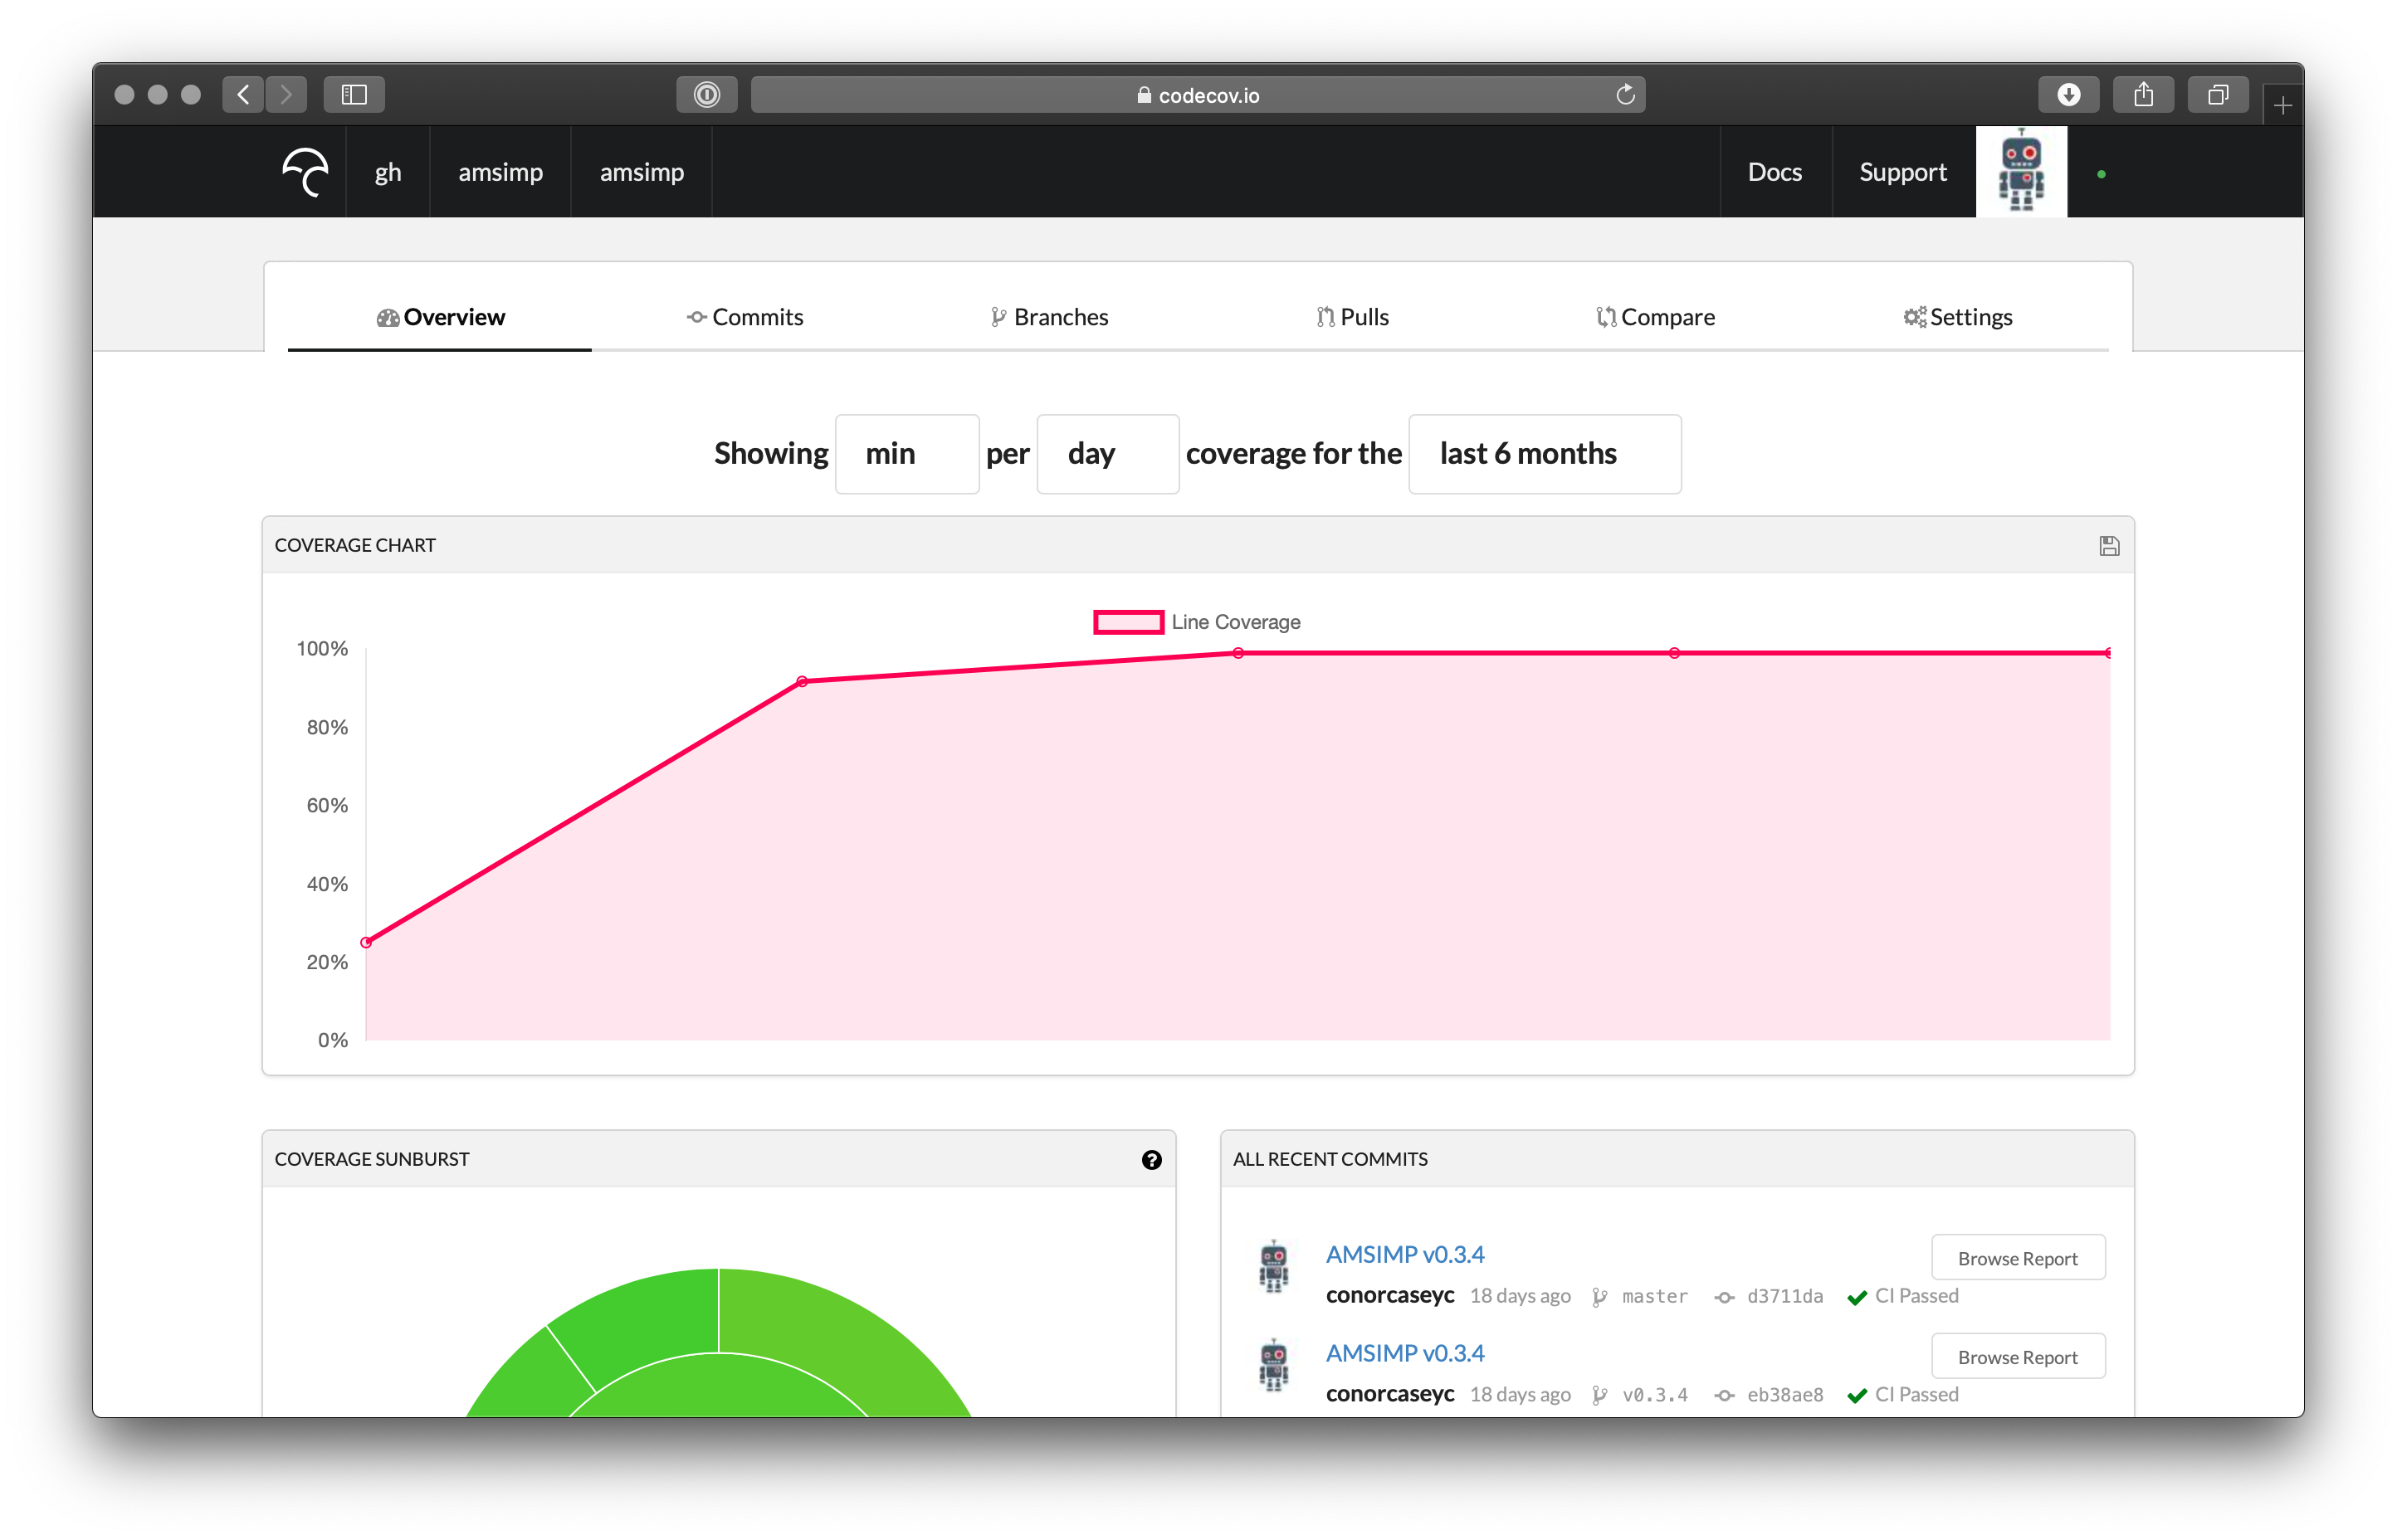
\includegraphics[width=.8\linewidth]{Images/codecov.png}
    \caption{A screenshot of the coverage benchmark results for the software on Codecov.}
    \label{codecov_image}
\end{figure}